\documentclass[lecture.tex]{subfiles}

\begin{document}

\exercice{}
\video{https://youtu.be/xYCddTAVD0g}
\enonce{rdm-0034}{}

\begin{center}
  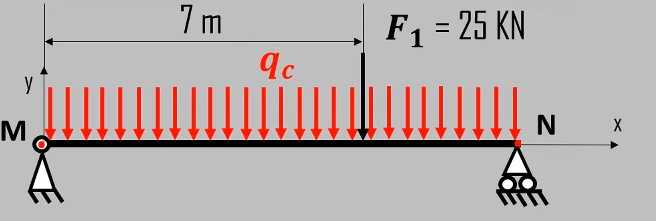
\includegraphics[scale=0.5]{figA0034.png}
\end{center}

La longueur de la poutre $MN$ est $L=12 \ m$. On a $q_{c}=25 \ kN / m$, qui est une charge linéaire.

\begin{enumerate}
    \item Déterminer les réactions de la poutre.
    \item Dessiner les diagrammes de l'effort tranchant et du moment fléchissant tout au long de la poutre.
\end{enumerate}

\finenonce{rdm-0034}
\finexercice


\end{document}
